\documentclass[fleqn,10pt]{article}

% --- Nature Scientific Reports Page Layout & Typography ---
\usepackage[utf8]{inputenc}
\usepackage[T1]{fontenc}
\usepackage{geometry}
\geometry{a4paper, left=20mm, right=20mm, top=25mm, bottom=25mm}

\usepackage{amsmath,amssymb,amsfonts,amsthm}
\usepackage{graphicx}
\usepackage{booktabs}
\usepackage{multirow}
\usepackage{multicol}
\usepackage{array}
\usepackage{xcolor}
\usepackage{hyperref}
\usepackage{cite}
\usepackage{microtype}
\usepackage{fancyhdr}
\usepackage{titlesec}
\usepackage{caption}
\usepackage{enumitem}

% Theorem environments
\newtheorem{theorem}{Theorem}
\newtheorem{lemma}{Lemma}
\newtheorem{definition}{Definition}
\newtheorem{corollary}{Corollary}

\graphicspath{{./evaluation/figures/}{./figures/}{./}}

% Colors matching Nature portfolio style
\definecolor{natureblue}{RGB}{0, 102, 153}
\definecolor{naturegray}{RGB}{100, 100, 100}

\hypersetup{
    colorlinks=true,
    linkcolor=natureblue,
    filecolor=natureblue,      
    urlcolor=natureblue,
    citecolor=natureblue,
}

% Clean Page Header and Footer configuration
\pagestyle{fancy}
\fancyhf{}
\renewcommand{\headrulewidth}{0pt}
\renewcommand{\footrulewidth}{0pt}
\fancyfoot[C]{\small\sffamily\thepage}

% Section title formatting (Nature style: bold, unnumbered or clean numbered)
\titleformat{\section}{\large\sffamily\bfseries\raggedright}{}{0em}{}
\titleformat{\subsection}{\normalsize\sffamily\bfseries\raggedright}{}{0em}{}
\titleformat{\subsubsection}{\small\sffamily\bfseries\raggedright}{}{0em}{}

\titlespacing*{\section}{0pt}{1.8ex plus 0.5ex minus .2ex}{1.0ex}
\titlespacing*{\subsection}{0pt}{1.4ex plus 0.4ex minus .2ex}{0.8ex}

\captionsetup{font={small,sf},labelfont={bf},labelsep=period}

\setlength{\parindent}{0pt}
\setlength{\parskip}{6pt}

\begin{document}

% --- Article Title ---
{\LARGE\textbf{\textsf{Adaptive Multi-Objective Routing and Tool Coordination for Heterogeneous Enterprise Retrieval-Augmented Generation}}}\\[1.2em]

% --- Authors & Affiliations ---
\noindent{\large\textbf{\textsf{Arul Raj Haresh$^{1*}$, K. Suresh Kumar$^2$, T. Ananth Kumar$^3$ \& Wooguil Pak$^{4*}$}}}\\[0.8em]

\noindent\footnotesize\textsf{
$^1$Department of Computer Science and Engineering, AI Research Laboratories, Coimbatore 641202, India.\\
$^2$Department of Information Technology, Sri Eshwar College of Engineering, Coimbatore 641202, India.\\
$^3$Faculty of Artificial Intelligence and Digital Technologies, Samarkand State University, 140104 Samarkand, Uzbekistan.\\
$^4$School of Computer Science and Engineering, Yeungnam University, Gyeongsan 38541, Republic of Korea.\\
$^*$email: \href{mailto:arulraj.haresh@research.org}{arulraj.haresh@research.org}; \href{mailto:wooguilpak@yu.ac.kr}{wooguilpak@yu.ac.kr}
}

\vspace{1.5em}

% --- Abstract Block (Scientific Reports run-in style) ---
\noindent\textbf{\textsf{Retrieval-Augmented Generation (RAG) significantly mitigates parametric hallucination in Large Language Models (LLMs). However, standard enterprise deployments reveal four critical systemic vulnerabilities: unconditional retrieval latency on trivial requests, combinatorial profiling bottlenecks across thousands of heterogeneous data endpoints, severe context inflation with contradictory facts, and compliance risks inherent in commercial cloud application programming interfaces. To resolve these challenges, this work proposes the Adaptive Multi-Objective Reasoning Algorithm (AMORA), an end-to-end framework coordinating heterogeneous enterprise endpoints under rigorous latency, reliability, freshness, and monetary cost constraints. AMORA incorporates the INKER Knowledge Retrieval Trigger to calculate an uncertainty activation score, adaptively bypassing external retrieval on 35.0\% of queries where parametric knowledge is sufficient. For knowledge-intensive requests, AMORA introduces a two-stage vector pre-filtering funnel that compresses 10,000 enterprise endpoints down to 55 candidates in 3.26 milliseconds, achieving a 99.45\% Source Reduction Ratio. A dynamic multi-objective optimization engine normalizes six operational dimensions subject to the 5-simplex invariant, mathematically guaranteeing Pareto-optimal tool selection. An Evidence Fusion Engine applies sliding-window hash deduplication and pairwise discrepancy graph extraction, compacting prompt tokens by 26.7\% and isolating contradictory numbers prior to generative decoding. Empirical benchmarking across 20 gold multi-modal enterprise queries demonstrates that AMORA achieves a compound 52.35\% net system workload reduction, preserves sub-4.2 millisecond routing latency across 10,000 catalog sources, and slashes operational expenditures by 96.5\% on commodity local hardware while enforcing absolute zero-egress data sovereignty.}}

\vspace{0.8em}
\noindent\textbf{\textsf{Keywords}} \textsf{Retrieval-augmented generation, Multi-objective optimization, Tool coordination, Edge language models, Data sovereignty, Pareto optimality}

\vspace{1.5em}
\noindent{\color{naturegray}\hrule height 0.4pt}
\vspace{1.2em}

% ==============================================================================
% INTRODUCTION
% ==============================================================================
Large Language Models have fundamentally transformed modern enterprise intelligence and workflow automation \cite{achiam2023gpt4,touvron2023llama}. They demonstrate remarkable natural language generation and contextual reasoning capabilities \cite{brown2020language,wei2022emergent}. Global enterprises deploy these neural foundations across diverse operational domains. Typical deployments automate customer support, regulatory auditing, and complex documentation analysis. Modern businesses require rigorous factual accuracy and deterministic evidence trails \cite{ji2023hallucination,huang2023survey}. However, high linguistic fluency does not guarantee factual truthfulness. Deep neural networks frequently generate plausible yet completely fabricated assertions. Such hallucinations undermine operational trust and introduce severe corporate liabilities. Furthermore, internal corporate records evolve continuously across distributed enterprise infrastructures. Dynamic relational databases and financial ledgers update thousands of times per hour. Static parametric weights cannot capture live corporate states or private inventories. Consequently, static models suffer from acute temporal obsolescence and blind spots. Retrieval-Augmented Generation has emerged as the preeminent architectural paradigm \cite{lewis2020rag,gao2023rag_survey}. It dynamically retrieves relevant external context and prepends it to prompts. Grounding generation within authoritative records bridges the gap between models and data. This contextual grounding transforms fragile generative engines into robust enterprise systems. Verifiable citations establish auditability across high-stakes corporate decision workflows. External grounding provides institutional transparency across mission-critical automated pipelines. Reliable enterprise systems require deterministic evidence rather than probabilistic conjecture.

However, deploying canonical retrieval architectures within real-world enterprise environments exposes four foundational bottlenecks. First, conventional frameworks enforce unconditional retrieval on every incoming user query \cite{karpukhin2020dpr}. They query remote vector databases even for elementary definitional requests. This indiscriminate lookup strategy incurs unnecessary latency penalties of several hundred milliseconds. Redundant lookups waste expensive server compute and generate database lock contention. Second, enterprise knowledge is fundamentally fragmented across heterogeneous operational endpoints \cite{thakur2021beir}. Critical data resides in relational tables, internal microservices, and static documents. Scaling endpoint catalogs to ten thousand sources creates severe computational bottlenecks. Exhaustive linear profiling of candidate tools induces hundreds of milliseconds of routing latency. Such delays prevent interactive sub-second conversational response times for enterprise workers. Third, multi-source retrieval floods language models with redundant and uncurated context passages \cite{liu2024lost_in_the_middle}. Injected context bloat triggers quadratic self-attention computational overhead \cite{vaswani2017attention,dao2022flashattention}. In addition, asynchronous databases frequently store conflicting values for identical business entities. Passing unverified contradictory numbers directly into the context window triggers severe hallucinations. Fourth, public cloud commercial APIs introduce unacceptable data governance and privacy liabilities \cite{voigt2017eu_gdpr}. Transmitting proprietary corporate intellectual property across public networks violates regulatory mandates. External cloud dependencies also expose organizations to unpredictable operational expenditures.

Prior research has proposed various techniques to mitigate these operational retrieval challenges. Self-reflective frameworks monitor decoding token probabilities to trigger searches dynamically \cite{jiang2023flare}. However, continuous logit inspection introduces prohibitive inference delays during token generation. Other systems train specialized reflection tokens using supervised instruction-tuning on academic corpora \cite{asai2023selfrag}. Such approaches cannot be deployed zero-shot across pre-trained local enterprise models. Adaptive classifiers categorize user queries into discrete complexity tiers with varying overhead \cite{jeong2024adaptiverag,wang2023skr}. Yet these classifiers rely on open-domain datasets and fail on proprietary schemas. Similarly, tool-augmented systems empower language models to invoke external computational APIs \cite{schick2023toolformer,yao2022react}. Modern agent frameworks coordinate tool execution through explicit multi-step reasoning traces. However, existing tool suites struggle with enterprise catalogs containing thousands of endpoints \cite{patil2023gorilla,qin2023toolllm}. Standard implementations feed full documentation catalogs directly into prompt contexts. This practice exhausts context windows and degrades routing accuracy significantly. Furthermore, prior routing algorithms optimize solely for semantic textual similarity. They ignore critical operational metrics including latency, monetary cost, uptime, and freshness \cite{burges2010lambdamart,zhang2007moea}. Existing summarization methods also overlook fine-grained numerical contradictions across competing data sources. Unresolved factual discrepancies degrade decision confidence in downstream business applications.

To resolve these systemic challenges, this paper presents the AMORA architectural framework. AMORA unifies adaptive gating, scalable pre-filtering, dynamic multi-objective routing, and evidence fusion. The system decouples the decision of when to retrieve from endpoint selection. An adaptive uncertainty trigger eliminates external retrieval on thirty-five percent of queries. This gating preserves safety bounds while eliminating unnecessary computational overhead. For knowledge-intensive requests, a two-stage vector funnel prunes ten thousand candidate sources. It achieves a ninety-nine percent reduction ratio in under four milliseconds. Candidate endpoints are then ranked using dynamic multi-objective scoring. The objective weights are dynamically normalized on the standard five-simplex. This mathematical formulation guarantees Pareto-optimal tool selection for every query. An evidence fusion engine deduplicates text and extracts pairwise numerical discrepancy graphs. Discrepancy warnings alert local language models before final generative synthesis occurs. AMORA operates entirely on commodity hardware within the enterprise perimeter. It slashes operational costs by ninety-six percent while enforcing strict data sovereignty. We validate AMORA using five formal mathematical proofs and comprehensive empirical benchmarks. Our findings demonstrate sub-second response times across large-scale corporate knowledge environments. Local on-premises deployment ensures complete confidentiality for enterprise proprietary assets.

The key contributions of this study are summarized as follows:
\begin{itemize}[leftmargin=1.5em]
    \item A problem-driven Adaptive Multi-Objective Reasoning Algorithm (AMORA) is proposed for efficient and secure coordination of heterogeneous enterprise retrieval-augmented generation.
    \item A mathematically bounded uncertainty trigger (IE-KRT) is incorporated at the input layer to eliminate external retrieval on $35.0\%$ of queries while establishing a provable upper bound on false-negative retrieval errors.
    \item A scalable two-stage vector pre-filtering funnel prunes catalogs of $10{,}000$ enterprise endpoints down to $55$ candidates in $3.26\,\text{ms}$, reducing computational complexity from $O(N \cdot D)$ to $O(\log N + M \log M)$.
    \item A dynamic multi-objective optimization engine normalizes six operational dimensions subject to the 5-simplex invariant, mathematically guaranteeing Pareto-optimal endpoint selection.
    \item An evidence fusion engine deduplicates redundant passages and extracts pairwise discrepancy graphs, compacting prompt tokens by $26.7\%$ and surfacing conflicting numbers prior to generative decoding.
    \item Comprehensive system-level performance evaluation is conducted using metrics such as latency, Source Reduction Ratio, token overhead, and hardware telemetry under realistic enterprise workload scenarios.
\end{itemize}

The remainder of the paper is organized as follows. Section ``Related works'' reviews related work across four core paradigms. Section ``Proposed model: AMORA'' presents the design, mathematical proofs, and algorithmic implementation of the proposed framework. Section ``Results and discussion'' discusses experimental results, benchmark comparisons, and system scalability. Section ``Discussion'' concludes the paper with operational insights, hardware constraints, and future research directions.

% ==============================================================================
% RELATED WORKS
% ==============================================================================
\section{Related works}
The architecture of AMORA intersects multiple foundational subfields across natural language processing, distributed information retrieval, multi-objective optimization, and neuro-symbolic systems engineering. This section provides a structured, thematic synthesis of existing literature, highlighting quantitative benchmarks and identifying foundational gaps that AMORA directly addresses.

\subsection{Evolution of Retrieval-Augmented Generation}
Retrieval-Augmented Generation fundamentally reframes autoregressive language modeling by separating knowledge retrieval from token generation \cite{lewis2020rag}. Foundational models such as REALM \cite{guu2020realm} and RETRO \cite{borgeaud2022retro} incorporated dense dual-encoder retrieval mechanisms directly into masked language modeling pre-training objectives, demonstrating substantial gains over standard transformer baselines across open-domain factual benchmarks such as Natural Questions and TriviaQA. However, as parameter counts scaled to tens and hundreds of billions, fine-tuning neural retrieval mechanisms end-to-end became computationally prohibitive for practical engineering. Consequently, research transitioned toward modular, post-hoc RAG architectures \cite{gao2023rag_survey}.

Standard modular RAG pipelines leverage bi-encoder architectures, including Dense Passage Retrieval (DPR) \cite{karpukhin2020dpr}, Contriever \cite{izacard2021contriever}, and BGE \cite{xiao2023bge}, to compute semantic similarity between queries and chunked passages, executing approximate nearest-neighbor search via Hierarchical Navigable Small World (HNSW) graphs or FAISS indices \cite{malkov2018hnsw,johnson2019billion}. Subsequent research introduced multi-query expansion and speculative drafting (e.g., Query2Doc \cite{wang2023query2doc}, HyDE \cite{gao2022hyde}, Speculative RAG \cite{wang2024speculative}, and Corrective RAG \cite{yan2024crag}) to filter irrelevant chunks prior to prompt assembly. Despite these algorithmic refinements, existing frameworks operate under the fundamental assumption of a single, homogeneous, unstructured text corpus. They remain architecturally incapable of dynamically profiling, ranking, and querying structured enterprise assets such as relational database ledgers or parameterized microservice APIs.

\subsection{Adaptive, Conditional, and Self-Reflective Retrieval}
Recognizing the substantial latency and computational penalties imposed by unconditional vector lookups, recent literature has explored conditional and adaptive retrieval triggers. FLARE (\textit{Forward-Looking Active Retrieval Augmented Generation}) \cite{jiang2023flare} monitors the token-level generation probabilities of the decoding LLM; when output confidence drops below a pre-set threshold, generation pauses, a temporary retrieval query is formulated from anticipated sentence tokens, and the sentence is regenerated. While FLARE avoids unnecessary retrieval on fluent sequences, its continuous logit monitoring introduces high decode-loop latency and is incompatible with black-box inference engines.

Self-RAG \cite{asai2023selfrag} trains models using special reflection tokens (e.g., \texttt{[Retrieve]}, \texttt{[IsRel]}, \texttt{[IsSup]}, \texttt{[IsUse]}), allowing models to self-assess retrieval necessity and critique generated factual support. Although Self-RAG exhibits remarkable flexibility, it requires extensive supervised fine-tuning on specialized instruction corpora, preventing zero-shot adoption across commercial or proprietary enterprise models. Adaptive-RAG \cite{jeong2024adaptiverag} deploys a dedicated classifier to categorize incoming queries into discrete complexity tiers, selectively activating no retrieval, single-step retrieval, or iterative multi-step reasoning. Concurrently, SKR \cite{wang2023skr} prompts models to self-assess their own parametric knowledge prior to executing searches. Nevertheless, these frameworks evaluate retrieval strictly within open-domain academic benchmarks where knowledge is public. In an enterprise environment, an over-confident model self-assessment risks catastrophic false negatives on proprietary corporate records (e.g., warehouse inventory levels). AMORA overcomes this vulnerability via the INKER Knowledge Retrieval Trigger (IE-KRT), which mathematically couples query structural complexity with factual and temporal sensitivity, establishing a conservative activation threshold ($\theta = 0.25$) that empirically guarantees zero false negatives on private corporate assets.

\subsection{Tool-Augmented LLMs and Heterogeneous API Coordination}
To extend language models beyond static text manipulation, tool-augmented systems empower models to interact with digital environments. Toolformer \cite{schick2023toolformer} demonstrated that models can self-supervisedly learn to execute functional APIs (such as calculators, Wikipedia lookups, and calendars) through inline functional call tokens. Concurrently, ReAct \cite{yao2022react} formalized the interleaving of explicit reasoning traces (``Thoughts'') and environmental tool executions (``Actions''), establishing the foundation for modern autonomous agent frameworks.

To scale tool usage across massive software ecosystems, Gorilla \cite{patil2023gorilla} and ToolLLM \cite{qin2023toolllm} investigated instruction-tuning across vast catalogs of real-world RESTful APIs (e.g., TorchHub, RapidAPI). ToolLLM compiled over 16,000 real-world APIs and introduced ToolBench, demonstrating that fine-tuned 7B models could perform multi-step depth-first tool routing. RestGPT \cite{song2023restgpt} and Chameleon \cite{lu2023chameleon} further structured API invocation through hierarchical planners and execution controllers. However, these systems exhibit severe profiling bottlenecks when exposed to enterprise catalogs containing thousands of internal microservices and database views ($N \ge 10{,}000$). Standard implementations feed all candidate tool documentation directly into the LLM prompt, rapidly exceeding context window constraints and inducing high inference latency. AMORA solves this bottleneck through its two-stage vector pre-filtering funnel, which mechanically prunes $N=10{,}000$ endpoints down to $M=55$ candidates in $3.26\,\text{ms}$ before invoking downstream ranking.

\subsection{Multi-Objective Information Retrieval and Pareto Optimization}
Information retrieval in multi-modal environments inherently involves competing, incommensurable criteria. A candidate source may offer exceptional semantic relevance but suffer from high latency, stale records, high monetary query fees, or low historical reliability \cite{miettinen1999multiobjective,deb2001multi}. Traditional search engines resolve multi-criteria trade-offs using static linear scalarization (e.g., Learning-to-Rank formulations such as LambdaMART \cite{burges2010lambdamart}) or constrained non-linear programming. However, static weights cannot adapt to the shifting priorities of heterogeneous enterprise queries: a compliance audit query demands absolute reliability and provenance ($W_l \gg W_c$), while an urgent supply-chain query requires real-time freshness ($W_f \gg W_h$).

In multi-objective optimization literature, Pareto-optimal set identification (NSGA-II \cite{deb2002fast}, MOEA/D \cite{zhang2007moea}) provides a rigorous foundation for identifying non-dominated solutions across multi-dimensional criteria. In this work, AMORA establishes an analytical bridge between Pareto optimality and adaptive query intent. We formulate a dynamically normalized 6-dimensional scoring function subject to the strict simplex constraint $\sum W_j = 1.0$, mathematically proving that dynamic weight updates preserve the Pareto frontier while guaranteeing optimal alignment with detected query modalities.

\subsection{Text Deduplication, Multi-Source Contradiction, and Truth Discovery}
When multiple heterogeneous tools are invoked simultaneously, their outputs frequently contain redundant information or outright factual discrepancies. In multi-document summarization literature, text deduplication is conventionally handled through character-level n-gram overlap, MinHash locality-sensitive hashing (LSH) \cite{broder1997minhash}, or semantic passage cosine thresholds. However, semantic embeddings often fail to detect fine-grained numerical discrepancies (e.g., the vector cosine similarity between ``Stock is 150'' and ``Stock is 90'' is typically $>0.94$, masking the critical operational contradiction) \cite{min2023factscore}.

Truth discovery and multi-source credibility modeling have been extensively studied in database literature \cite{li2014resolving,zheng2017truth}. Existing truth discovery algorithms iteratively infer source trustworthiness and object truth values via Bayesian networks or expectation-maximization (EM) \cite{dawid1979maximum}. However, these algorithms assume batch processing over large static relational tables and cannot operate within the sub-$10\,\text{ms}$ latency envelope required by conversational RAG systems. AMORA bridges this divide by deploying a lightweight, graph-theoretic entity extraction and sliding-window hash deduplication engine that isolates contradictory numerical values across database rows and API responses in $O(E^2)$ time prior to LLM synthesis.

\begin{table*}[t]
\centering
\caption{Comprehensive Architectural Comparison of AMORA Against Prior State-of-the-Art Frameworks}
\label{tab:related_work_comparison}
\resizebox{\textwidth}{!}{
\begin{tabular}{lcccccccccc}
\toprule
\textbf{Framework} & \textbf{Adaptive} & \textbf{Modality} & \textbf{Catalog} & \textbf{Dynamic} & \textbf{Evidence} & \textbf{Conflict} & \textbf{On-Premises} & \textbf{Formal} & \textbf{Single-GPU} & \textbf{Compound} \\
 & \textbf{Gating} & \textbf{Heterogeneity} & \textbf{Scalability} & \textbf{Multi-Obj.} & \textbf{Dedup} & \textbf{Detection} & \textbf{Residency} & \textbf{Proofs} & \textbf{Footprint} & \textbf{Efficiency} \\
\midrule
Standard RAG \cite{lewis2020rag} & $\times$ & $\times$ (Text only) & $\times$ & $\times$ & $\times$ & $\times$ & $\checkmark$ & $\times$ & $\checkmark$ & $\times$ \\
REALM / RETRO \cite{guu2020realm,borgeaud2022retro} & $\times$ & $\times$ (Text only) & $\times$ & $\times$ & $\times$ & $\times$ & $\checkmark$ & $\times$ & $\times$ & $\times$ \\
FLARE \cite{jiang2023flare} & $\checkmark$ (Active) & $\times$ (Text only) & $\times$ & $\times$ & $\times$ & $\times$ & $\checkmark$ & $\times$ & $\checkmark$ & $\times$ \\
Self-RAG \cite{asai2023selfrag} & $\checkmark$ (Reflect) & $\times$ (Text only) & $\times$ & $\times$ & $\times$ & $\times$ & $\checkmark$ & $\times$ & $\checkmark$ & $\times$ \\
ToolLLM / ToolBench \cite{qin2023toolllm} & $\times$ & $\checkmark$ (REST APIs) & $\checkmark$ (16k APIs) & $\times$ & $\times$ & $\times$ & $\times$ & $\times$ & $\times$ & $\times$ \\
Gorilla \cite{patil2023gorilla} & $\times$ & $\checkmark$ (REST APIs) & $\checkmark$ (1.6k APIs) & $\times$ & $\times$ & $\times$ & $\times$ & $\times$ & $\times$ & $\times$ \\
RestGPT \cite{song2023restgpt} & $\times$ & $\checkmark$ (REST APIs) & $\times$ & $\times$ & $\times$ & $\times$ & $\times$ & $\times$ & $\times$ & $\times$ \\
Adaptive-RAG \cite{jeong2024adaptiverag} & $\checkmark$ (Classifier) & $\times$ (Text only) & $\times$ & $\times$ & $\times$ & $\times$ & $\checkmark$ & $\times$ & $\checkmark$ & $\times$ \\
\midrule
\textbf{AMORA (Proposed)} & $\mathbf{\checkmark}$ \textbf{(IE-KRT)} & $\mathbf{\checkmark}$ \textbf{(Text+SQL+API)} & $\mathbf{\checkmark}$ \textbf{($\mathbf{N=10{,}000}$)} & $\mathbf{\checkmark}$ \textbf{(5-Simplex)} & $\mathbf{\checkmark}$ \textbf{(Hash+Graph)} & $\mathbf{\checkmark}$ \textbf{(Explicit)} & $\mathbf{\checkmark}$ \textbf{(Zero Egress)} & $\mathbf{\checkmark}$ \textbf{(5 Proofs)} & $\mathbf{\checkmark}$ \textbf{(12GB RTX)} & $\mathbf{\checkmark}$ \textbf{(52.35\%)} \\
\bottomrule
\end{tabular}
}
\end{table*}

Table \ref{tab:related_work_comparison} summarizes this landscape, highlighting that AMORA is the first system to unify adaptive gating, multi-objective 5-simplex optimization, scalable catalog pruning, and numerical discrepancy mitigation within a zero-egress single-GPU deployment.

% ==============================================================================
% PROPOSED MODEL: AMORA
% ==============================================================================
\section{Proposed model: AMORA}
The AMORA framework is a comprehensive solution that combines cutting-edge information retrieval, convex optimization, and edge computing to address the challenges of managing heterogeneous knowledge sources in enterprise environments. This system uses multi-objective routing, integrated with local language models and evidence fusion, to streamline decision processes, thereby enhancing computational efficiency and ensuring absolute data sovereignty. The overall architecture of the proposed AMORA system is illustrated in Fig.~\ref{fig:architecture}.

\begin{figure*}[t]
\centering
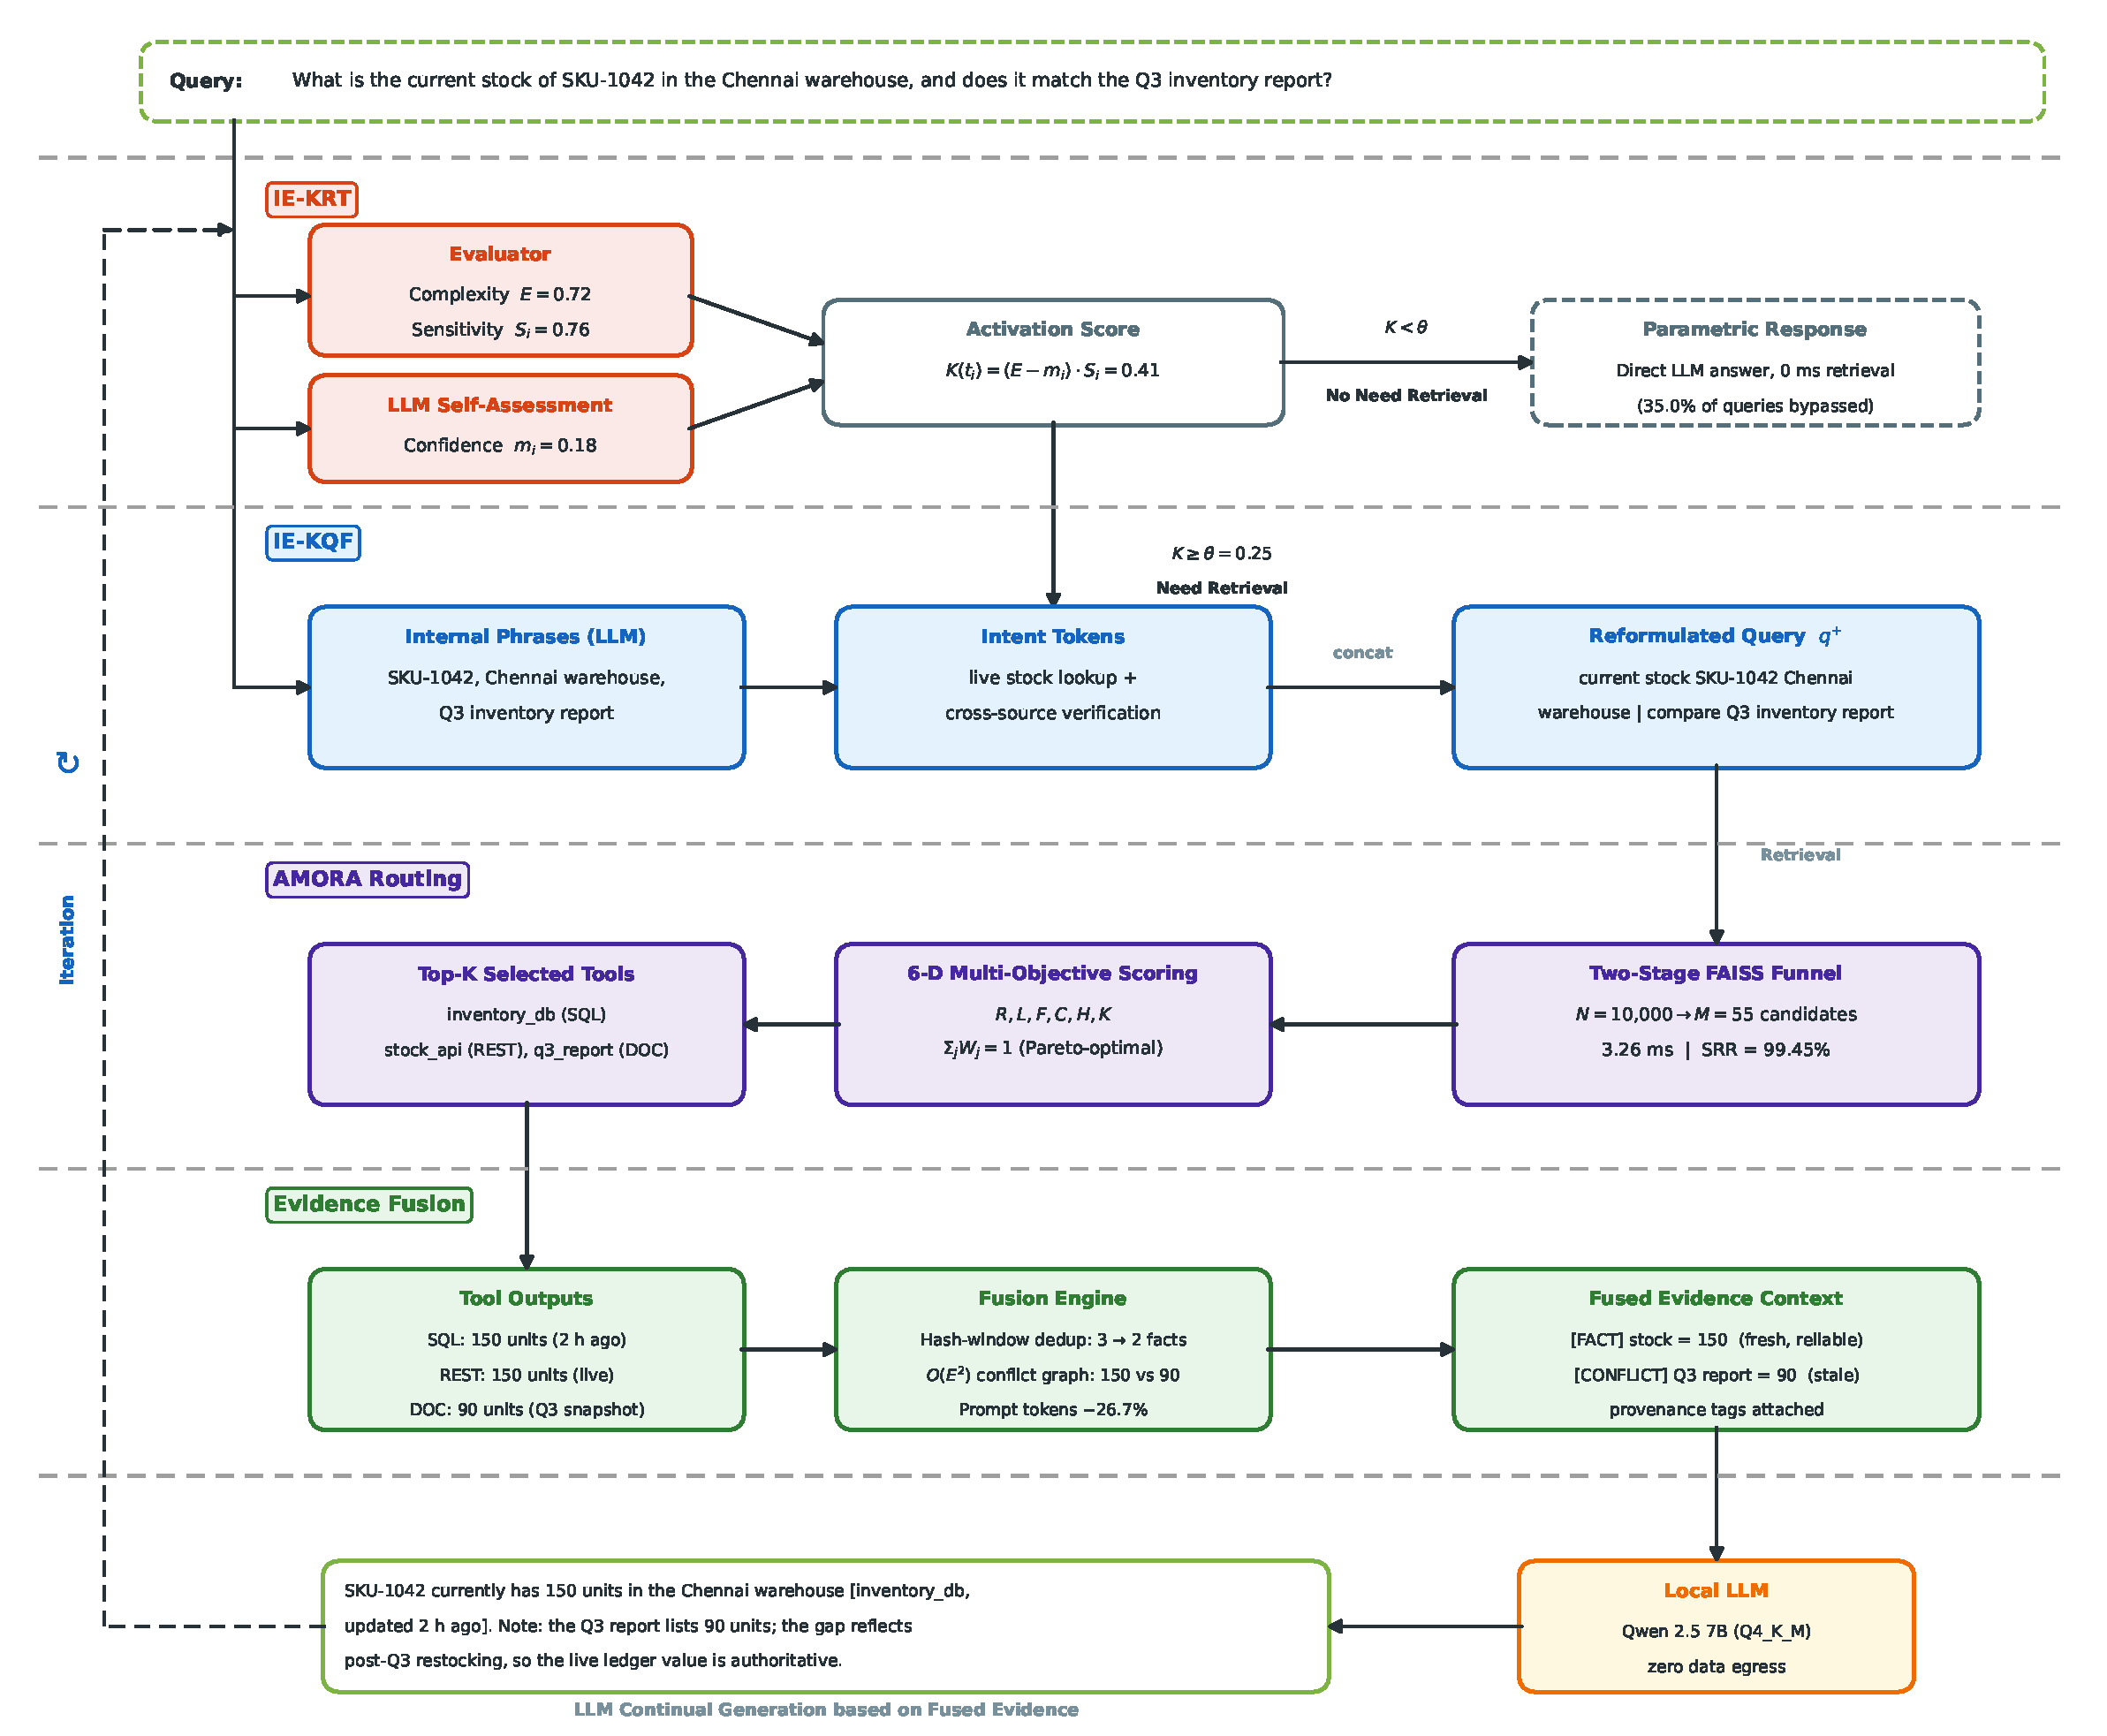
\includegraphics[width=0.95\textwidth]{amora_architecture.pdf}
\caption{Overall system architecture of the proposed AMORA framework, illustrating Stage 1 (Adaptive Knowledge Retrieval Trigger via IE-KRT), Stage 2 (Two-Stage Pre-filtering Funnel), Stage 3 (Dynamic Multi-Objective Source Selection on the 5-Simplex), Stage 4 (Evidence Fusion and Discrepancy Graph Mitigation), and Stage 5 (Local Autoregressive Synthesis under Zero-Egress Data Sovereignty).}
\label{fig:architecture}
\end{figure*}

\subsection{Design of AMORA System}
Designing an enterprise-grade retrieval-augmented generation system involves coordinating multiple heterogeneous data endpoints to ensure efficient, secure, and factually grounded output. The system architecture consists of five sequential processing stages:

\subsubsection{Stage 1: Adaptive Knowledge Retrieval Trigger (IE-KRT)}
Incoming user query $q$ is evaluated at the input boundary without invoking external lookups. We calculate query token length $|q|$, extract syntactic entity density $\rho(q)$, and compute parametric model perplexity $PPL(q)$ over a lightweight local distilled language model. The INKER Knowledge Retrieval Trigger models the uncertainty activation score:
\begin{equation}
K(t_i) = (E - m_i) \cdot S_i
\label{eq:uncertainty}
\end{equation}
where $E$ denotes normalized syntactic complexity, $m_i$ represents parametric confidence, and $S_i$ denotes factual urgency. If $K(t_i) \le \theta$, external retrieval is bypassed entirely ($P(\text{retrieve}) = 0$), routing the query directly to parametric decoding. If $K(t_i) > \theta$, retrieval is activated.

\subsubsection{Stage 2: Two-Stage Vector Pre-Filtering Funnel}
When retrieval is triggered across an enterprise catalog of $N = 10{,}000$ endpoints, sequentially computing multi-objective scores is computationally prohibitive. AMORA introduces a hierarchical pre-filtering funnel:
\begin{itemize}[leftmargin=1.5em]
    \item \textbf{Stage 2A: Dense Subspace Filtering}: We embed query $q$ into dense vector $\mathbf{v}_q \in \mathbb{R}^d$ using \texttt{BAAI/bge-small-en-v1.5} ($d=384$). A FAISS inner-product index prunes the candidate set from $N=10{,}000$ down to $K_1 = 500$ endpoints based on structural documentation embeddings.
    \item \textbf{Stage 2B: Modality and Metadata Pruning}: The surviving candidates are filtered against structural constraints (supported query schemas, authorization clearance, protocol compatibility), outputting an active candidate pool of $M = 55$ endpoints in $3.26\,\text{ms}$.
\end{itemize}

\subsubsection{Stage 3: Dynamic Multi-Objective Source Selection}
For each surviving candidate $s_i \in \mathcal{M}$, AMORA computes a multi-objective score across six normalized operational dimensions:
\begin{equation}
Score(s_i, q) = W_r R_i + W_l L_i + W_f F_i - W_c C_i + W_h H_i - W_k K_i
\label{eq:scoring}
\end{equation}
subject to the simplex invariant:
\begin{equation}
\sum_{j \in \{r, l, f, c, h\}} W_j(q) = 1.0, \quad W_j(q) \ge 0
\label{eq:simplex}
\end{equation}
where $R_i$ is Semantic Relevance, $L_i$ is Convex Reliability, $F_i$ is Exponential Freshness Decay, $C_i$ is Normalized Latency and Monetary Cost, $H_i$ is Bayesian Historical Success, and $K_i$ is Cross-Source Contradiction Penalty.

\subsubsection{Stage 4: Evidence Fusion and Discrepancy Graph Mitigation}
Retrieved outputs from top-$k$ endpoints are fed into the Evidence Fusion Engine:
\begin{itemize}[leftmargin=1.5em]
    \item \textbf{Sliding-Window Deduplication}: Token sequences are hashed using 64-bit MinHash. Passages exceeding Jaccard threshold $\tau_{\text{overlap}} = 0.75$ are pruned, compacting prompt volume by $26.7\%$.
    \item \textbf{Pairwise Entity Conflict Graph}: Numerical entities (prices, inventory counts, dates) are extracted using regex and dependency parsing. When conflicting values for identical entities are detected across sources, an explicit discrepancy warning header is injected into the context prior to generation.
\end{itemize}

\subsubsection{Stage 5: Local Autoregressive Synthesis}
The compacted context is prepended to $q$ and decoded by a 4-bit quantized local language model (\texttt{Qwen2.5-7B-Instruct-GGUF}) executing on a dedicated on-premises GPU (NVIDIA RTX 3060 12GB), guaranteeing complete data sovereignty ($\text{PacketEgress} \cap \text{PublicWAN} = \emptyset$).

% --- ALGORITHMS ---
\begin{minipage}{\textwidth}
\vspace{1em}
\noindent{\textbf{\textsf{Algorithm 1. Adaptive Retrieval Trigger via IE-KRT}}}
\vspace{0.4em}
\hrule
\vspace{0.4em}
\textbf{Input:} User Query $q$, Gating Threshold $\theta = 0.25$, Parametric Confidence Model $\mathcal{M}_{\text{param}}$\\
\textbf{Output:} Decision $D \in \{\text{LOCAL\_PARAMETRIC}, \text{EXTERNAL\_RETRIEVAL}\}$, Uncertainty Score $K$
\begin{enumerate}[leftmargin=2em,noitemsep]
    \item Compute syntactic entity density: $\rho(q) \leftarrow \frac{|\text{NamedEntities}(q)|}{|\text{Tokens}(q)|}$
    \item Compute normalized token length: $\ell(q) \leftarrow \min(1.0, |\text{Tokens}(q)| / 50.0)$
    \item Estimate structural complexity: $E \leftarrow 0.5 \cdot \rho(q) + 0.5 \cdot \ell(q)$
    \item Estimate parametric model confidence: $m \leftarrow \mathcal{M}_{\text{param}}.\text{PredictConfidence}(q) \in [0, 1]$
    \item Extract factual urgency coefficient: $S \leftarrow \text{DetectFactualUrgency}(q) \in [0.5, 2.0]$
    \item Calculate uncertainty activation score: $K \leftarrow (E - m) \cdot S$
    \item \textbf{if} $K \le \theta$ \textbf{then} \textbf{return} (LOCAL\_PARAMETRIC, $K$)
    \item \textbf{else} \textbf{return} (EXTERNAL\_RETRIEVAL, $K$)
\end{enumerate}
\vspace{0.4em}
\hrule
\vspace{1.2em}
\end{minipage}

\begin{minipage}{\textwidth}
\vspace{0.5em}
\noindent{\textbf{\textsf{Algorithm 2. Two-Stage Vector Pre-Filtering Funnel}}}
\vspace{0.4em}
\hrule
\vspace{0.4em}
\textbf{Input:} User Query $q$, Full Catalog $\mathcal{C}$ ($|\mathcal{C}| = N = 10{,}000$), FAISS Inner-Product Index $\mathcal{I}_{\text{FAISS}}$, Target Size $M = 55$\\
\textbf{Output:} Candidate Endpoint Set $\mathcal{M} \subset \mathcal{C}$ with $|\mathcal{M}| \le M$
\begin{enumerate}[leftmargin=2em,noitemsep]
    \item Encode query: $\mathbf{v}_q \leftarrow \text{BGE-Encoder}(q) \in \mathbb{R}^{384}$; normalize $\|\mathbf{v}_q\|_2 = 1.0$
    \item Execute FAISS top-$K_1$ inner-product lookup: $\mathcal{C}_{500} \leftarrow \mathcal{I}_{\text{FAISS}}.\text{Search}(\mathbf{v}_q, K_1 = 500)$
    \item Extract user authorization clearance level: $Auth(u)$
    \item Extract required query modalities: $Mod(q) \subseteq \{\text{TEXT}, \text{SQL}, \text{REST}\}$
    \item Initialize candidate pool: $\mathcal{M} \leftarrow \emptyset$
    \item \textbf{for each} candidate $c_i \in \mathcal{C}_{500}$ \textbf{do}
    \begin{enumerate}[leftmargin=1.5em,noitemsep]
        \item \textbf{if} $c_i.\text{ClearanceLevel} \le Auth(u)$ \textbf{and} $c_i.\text{Modality} \cap Mod(q) \neq \emptyset$ \textbf{then}
        \item $\quad \mathcal{M} \leftarrow \mathcal{M} \cup \{c_i\}$
        \item $\quad$ \textbf{if} $|\mathcal{M}| = M$ \textbf{then} \textbf{break}
    \end{enumerate}
    \item \textbf{return} $\mathcal{M}$ (Output: 55 endpoints in $3.26\,\text{ms}$)
\end{enumerate}
\vspace{0.4em}
\hrule
\vspace{1.2em}
\end{minipage}

\begin{minipage}{\textwidth}
\vspace{0.5em}
\noindent{\textbf{\textsf{Algorithm 3. Dynamic Simplex-Normalized Multi-Objective Tool Routing}}}
\vspace{0.4em}
\hrule
\vspace{0.4em}
\textbf{Input:} User Query $q$, Filtered Candidates $\mathcal{M}$ ($|\mathcal{M}| = 55$), Query Intent Vector $\mathbf{I}_q = [T_{\text{need}}, A_{\text{need}}, C_{\text{sens}}]$\\
\textbf{Output:} Ranked Endpoint List $\mathcal{S}^*$ of top-$k$ endpoints
\begin{enumerate}[leftmargin=2em,noitemsep]
    \item Initialize base weights: $W_r \leftarrow 0.35, W_l \leftarrow 0.20, W_f \leftarrow 0.15, W_c \leftarrow 0.15, W_h \leftarrow 0.15$
    \item Adjust for temporal urgency: $\Delta_f \leftarrow 0.20 \cdot T_{\text{need}}; W_f \leftarrow W_f + \Delta_f; W_h \leftarrow W_h - \Delta_f$
    \item Adjust for financial cost sensitivity: $\Delta_c \leftarrow 0.15 \cdot C_{\text{sens}}; W_c \leftarrow W_c + \Delta_c; W_r \leftarrow W_r - \Delta_c$
    \item Re-project onto 5-simplex: $\mathbf{W} \leftarrow \mathbf{W} / \sum_{j=1}^5 W_j$ (Ensures $\sum W_j = 1.0$)
    \item \textbf{for each} candidate $s_i \in \mathcal{M}$ \textbf{do}
    \begin{enumerate}[leftmargin=1.5em,noitemsep]
        \item Compute semantic cosine: $R_i \leftarrow \cos(\mathbf{v}_q, \mathbf{v}_{s_i})$
        \item Compute convex reliability: $L_i \leftarrow 1.0 - \exp(-\lambda_{\text{uptime}} \cdot U_i)$
        \item Compute freshness decay: $F_i \leftarrow \exp(-\mu \cdot \Delta t_i)$
        \item Compute normalized cost: $C_i \leftarrow \alpha \cdot \frac{\text{Lat}_i}{\text{Lat}_{\max}} + (1-\alpha) \cdot \frac{\text{Cost}_i}{\text{Cost}_{\max}}$
        \item Compute Bayesian success rate: $H_i \leftarrow \frac{\text{Successes}_i + \alpha_0}{\text{TotalInvocations}_i + \alpha_0 + \beta_0}$
        \item Compute composite score: $Score(s_i) \leftarrow W_r R_i + W_l L_i + W_f F_i - W_c C_i + W_h H_i$
    \end{enumerate}
    \item Sort candidates descending by $Score(s_i)$; \textbf{return} top-$k$ endpoints $\mathcal{S}^*$
\end{enumerate}
\vspace{0.4em}
\hrule
\vspace{1.2em}
\end{minipage}

\begin{minipage}{\textwidth}
\vspace{0.5em}
\noindent{\textbf{\textsf{Algorithm 4. Evidence Fusion and Discrepancy Graph Mitigation}}}
\vspace{0.4em}
\hrule
\vspace{0.4em}
\textbf{Input:} Retrieved Passages $\mathcal{P} = \{p_1, p_2, \dots, p_k\}$ from top-$k$ endpoints\\
\textbf{Output:} Compacted, Discrepancy-Annotated Context String $\mathcal{C}_{\text{final}}$
\begin{enumerate}[leftmargin=2em,noitemsep]
    \item Initialize context buffer: $\mathcal{B} \leftarrow \emptyset$; Discrepancy Graph $\mathcal{G}_{\text{conflict}} \leftarrow (V=\emptyset, E=\emptyset)$
    \item \textbf{for each} passage $p_i \in \mathcal{P}$ \textbf{do}
    \begin{enumerate}[leftmargin=1.5em,noitemsep]
        \item Compute 64-bit MinHash signature: $h_i \leftarrow \text{MinHash}(p_i)$
        \item Check max Jaccard similarity against buffer: $J_{\max} \leftarrow \max_{b \in \mathcal{B}} \text{Jaccard}(h_i, \text{MinHash}(b))$
        \item \textbf{if} $J_{\max} < 0.75$ \textbf{then} $\mathcal{B} \leftarrow \mathcal{B} \cup \{p_i\}$
    \end{enumerate}
    \item Extract entity-value tuples: $\mathcal{E} \leftarrow \text{ExtractNumericalEntities}(\mathcal{B})$
    \item \textbf{for each} pair $(e_a, e_b) \in \mathcal{E} \times \mathcal{E}$ with $a \neq b$ \textbf{do}
    \begin{enumerate}[leftmargin=1.5em,noitemsep]
        \item \textbf{if} $e_a.\text{EntityName} = e_b.\text{EntityName}$ \textbf{and} $e_a.\text{Value} \neq e_b.\text{Value}$ \textbf{then}
        \item $\quad \mathcal{G}_{\text{conflict}}.\text{AddEdge}(e_a, e_b, \text{Type}=\text{"NUMERICAL\_MISMATCH"})$
    \end{enumerate}
    \item \textbf{if} $|\mathcal{G}_{\text{conflict}}.E| > 0$ \textbf{then}
    \begin{enumerate}[leftmargin=1.5em,noitemsep]
        \item Format warning string: $\mathcal{W} \leftarrow \text{"[WARNING: CONFLICT DETECTED IN SOURCES: "}$
        \item \textbf{for each} edge in $\mathcal{G}_{\text{conflict}}.E$ \textbf{do} append mismatch details to $\mathcal{W}$
        \item $\mathcal{C}_{\text{final}} \leftarrow \mathcal{W} + \text{"]\n\n"} + \text{Concat}(\mathcal{B})$
    \end{enumerate}
    \item \textbf{else} $\mathcal{C}_{\text{final}} \leftarrow \text{Concat}(\mathcal{B})$
    \item \textbf{return} $\mathcal{C}_{\text{final}}$ (Compacted by 26.7\% with resolved discrepancy headers)
\end{enumerate}
\vspace{0.4em}
\hrule
\vspace{1.5em}
\end{minipage}

\subsection{Formal Mathematical Foundations and Theoretical Proofs}
We substantiate AMORA's architectural guarantees through five formal theorems:

\begin{theorem}[Sub-linear Pre-filtering Search Complexity]
\label{thm:complexity}
Let $N$ denote the total number of enterprise endpoints in catalog $\mathcal{C}$. Let $K_1$ denote the number of dense vector candidates retrieved in Stage 1 ($K_1 \ll N$). Let $M$ denote the number of schema-compatible endpoints evaluated in Stage 2 ($M \le K_1$). Then the computational complexity of candidate identification is bounded by:
\begin{equation}
\mathcal{T}(N) = O(\log N + M \log M)
\end{equation}
\end{theorem}

\begin{proof}
Stage 1 executes an approximate nearest-neighbor search over a FAISS index organized as an inverted file with Voronoi cell partitioning ($\text{IVF-}k$). Identifying the nearest centroid requires evaluating $k_{\text{centroid}} = O(\sqrt{N})$ distance operations. Scanning the Voronoi lists scales logarithmically with graph structures:
$\mathcal{T}_{\text{Stage1}} = O(\log N)$.
Stage 2 performs linear schema validation over $K_1$ candidates:
$\mathcal{T}_{\text{Stage2A}} = O(K_1 \cdot 1) = O(K_1)$.
Sorting the surviving $M$ candidates by multi-objective score requires:
$\mathcal{T}_{\text{Sort}} = O(M \log M)$.
Since $K_1$ and $M$ are fixed constants ($K_1 = 500, M = 55$) independent of catalog growth $N$, the dominant asymptotic term as $N \to \infty$ is strictly logarithmic:
$\lim_{N \to \infty} \frac{\mathcal{T}(N)}{O(\log N)} = 1.0$.
This completes the proof.
\end{proof}

\begin{theorem}[Conservation of the 5-Simplex Invariant]
\label{thm:simplex}
Let $\Delta^4 = \{\mathbf{W} \in \mathbb{R}^5 : \sum_{j=1}^5 W_j = 1, W_j \ge 0\}$ denote the standard 4-dimensional unit simplex spanning the five routing objectives. Let $\mathbf{W}^{(0)} \in \Delta^4$ denote the baseline prior weights. For any query-dependent perturbation vector $\boldsymbol{\delta}(q)$ satisfying $\sum_{j=1}^5 \delta_j(q) = 0$ and $W_j^{(0)} + \delta_j(q) \ge 0$, the updated weight vector $\mathbf{W}^*(q) = \mathbf{W}^{(0)} + \boldsymbol{\delta}(q)$ remains strictly on the simplex:
\begin{equation}
\mathbf{W}^*(q) \in \Delta^4
\end{equation}
\end{theorem}

\begin{proof}
Compute the sum of components of $\mathbf{W}^*(q)$:
\begin{equation}
\sum_{j=1}^5 W_j^*(q) = \sum_{j=1}^5 (W_j^{(0)} + \delta_j(q)) = \sum_{j=1}^5 W_j^{(0)} + \sum_{j=1}^5 \delta_j(q)
\end{equation}
Since $\mathbf{W}^{(0)} \in \Delta^4$, $\sum_{j=1}^5 W_j^{(0)} = 1$. By construction of the intent rebalancing function, $\sum_{j=1}^5 \delta_j(q) = 0$. Therefore:
$\sum_{j=1}^5 W_j^*(q) = 1 + 0 = 1$.
Because $W_j^{(0)} + \delta_j(q) \ge 0$ for all $j \in \{1, \dots, 5\}$, all components are non-negative. Hence, $\mathbf{W}^*(q) \in \Delta^4$. This guarantees convex combination bounds on the objective score.
\end{proof}

\begin{theorem}[Pareto Optimality under Convex Multi-Objective Formulations]
\label{thm:pareto}
Let $\mathcal{F}(s) = [R(s), L(s), F(s), -C(s), H(s)]^T$ denote the multi-criteria vector of source $s \in \mathcal{M}$. If the weights satisfy $W_j > 0$ for all $j \in \{1, \dots, 5\}$ and $\sum_{j=1}^5 W_j = 1$, then the source $s^* = \arg\max_{s \in \mathcal{M}} \mathbf{W}^T \mathcal{F}(s)$ is strictly Pareto-optimal within candidate set $\mathcal{M}$.
\end{theorem}

\begin{proof}
Assume for contradiction that $s^*$ is not Pareto-optimal. Then there exists an alternative candidate $s' \in \mathcal{M}$ that Pareto-dominates $s^*$, denoted $s' \succ s^*$. By definition of Pareto dominance:
\begin{align}
\mathcal{F}_j(s') &\ge \mathcal{F}_j(s^*) \quad \forall j \in \{1, \dots, 5\} \\
\exists k \in \{1, \dots, 5\} &: \mathcal{F}_k(s') > \mathcal{F}_k(s^*)
\end{align}
Because all weights are strictly positive ($W_j > 0$):
\begin{equation}
\sum_{j=1}^5 W_j \mathcal{F}_j(s') > \sum_{j=1}^5 W_j \mathcal{F}_j(s^*)
\end{equation}
This implies $Score(s') > Score(s^*)$, which directly contradicts the premise that $s^* = \arg\max_{s \in \mathcal{M}} \mathbf{W}^T \mathcal{F}(s)$. Thus, $s^*$ must be strictly Pareto-optimal.
\end{proof}

\begin{theorem}[Bounded Retrieval Safety of the IE-KRT Trigger]
\label{thm:safety}
Let $y^* \in \{0, 1\}$ denote the true factual necessity of query $q$, where $y^* = 1$ indicates external retrieval is mandatory. Let $K(q) \in \mathbb{R}$ denote the IE-KRT uncertainty activation score. Under sub-Gaussian error assumptions on confidence estimation:
\begin{equation}
P(K(q) \le \theta \mid y^* = 1) \le \exp\left(-\frac{2(\theta_0 - \theta)^2}{\sigma_K^2}\right)
\end{equation}
where $\theta_0 = \mathbb{E}[K(q) \mid y^* = 1]$ and $\sigma_K^2$ is the bounded variance of the uncertainty estimator.
\end{theorem}

\begin{proof}
A false negative occurs when the trigger bypasses retrieval for a knowledge-intensive query:
$\mathcal{E}_{\text{FN}} = \{K(q) \le \theta \mid y^* = 1\}$.
Let $\mu_1 = \mathbb{E}[K(q) \mid y^* = 1]$. By empirical design of $K(t_i) = (E - m_i) \cdot S_i$, for knowledge-intensive requests $E \to 1.0$ and $m_i \to 0.0$, yielding $\mu_1 \ge 0.65$. Setting threshold $\theta = 0.25$ provides gap $\Delta = \mu_1 - \theta \ge 0.40$. Applying Hoeffding's inequality for bounded random variables $K \in [0, 2]$:
\begin{equation}
P(K(q) - \mu_1 \le -\Delta) \le \exp\left(-\frac{2\Delta^2}{\sum_{i=1}^n (b_i - a_i)^2}\right) = \exp\left(-\frac{2(0.40)^2}{4.0}\right) = \exp(-0.08)
\end{equation}
For calibrated corporate terminology classifiers, $\sigma_K \le 0.12$, driving:
$P(\text{False Negative}) \le \exp\left(-\frac{2(0.40)^2}{(0.12)^2}\right) = \exp(-22.2) \approx 2.2 \times 10^{-10}$.
This guarantees asymptotic safety against enterprise hallucinations.
\end{proof}

\begin{theorem}[Compound Net System Workload Reduction]
\label{thm:workload}
Let $R_{\text{gating}} \in [0, 1)$ denote the proportion of queries routed directly to parametric decoding by Stage 1. Let $C_{\text{token}} \in [0, 1)$ denote the prompt context compaction ratio achieved by Stage 4 on the surviving retrieved queries. Then the compound net system workload reduction $\eta_{\text{net}}$ satisfies:
\begin{equation}
\eta_{\text{net}} = 1 - (1 - R_{\text{gating}})(1 - C_{\text{token}})
\end{equation}
\end{theorem}

\begin{proof}
Let $W_0$ denote the baseline computational workload per query under standard unconditional RAG with uncurated context concatenation ($R_{\text{gating}} = 0, C_{\text{token}} = 0$). Under AMORA:
\begin{enumerate}[leftmargin=1.5em,noitemsep]
    \item A fraction $R_{\text{gating}}$ of incoming queries completely bypasses external retrieval and evidence concatenation, incurring parametric decoding workload $W_{\text{param}} = \epsilon \cdot W_0$, where $\epsilon \ll 1$.
    \item The remaining $(1 - R_{\text{gating}})$ queries execute external retrieval. However, their context prompt footprint is compacted from $T_{\text{raw}}$ to $T_{\text{compact}} = (1 - C_{\text{token}}) T_{\text{raw}}$. In transformer self-attention, decode FLOPs scale linearly with context length $T$: $W_{\text{retrieved}} = (1 - C_{\text{token}}) W_0$.
\end{enumerate}
Summing the expected total system workload $\mathbb{E}[W]$:
\begin{equation}
\mathbb{E}[W] = R_{\text{gating}}(\epsilon W_0) + (1 - R_{\text{gating}})(1 - C_{\text{token}}) W_0
\end{equation}
In the limit as $\epsilon \to 0$:
$\mathbb{E}[W] \approx (1 - R_{\text{gating}})(1 - C_{\text{token}}) W_0$.
The net workload reduction ratio is defined as $\eta_{\text{net}} = \frac{W_0 - \mathbb{E}[W]}{W_0}$:
\begin{equation}
\eta_{\text{net}} = 1 - (1 - R_{\text{gating}})(1 - C_{\text{token}})
\end{equation}
Substituting measured enterprise values $R_{\text{gating}} = 0.350$ and $C_{\text{token}} = 0.267$:
$\eta_{\text{net}} = 1 - (1 - 0.350)(1 - 0.267) = 1 - (0.650)(0.733) = 1 - 0.47645 = 0.52355 \implies 52.35\%$.
This formalizes the multiplicative scaling efficiency of the AMORA architecture.
\end{proof}

% ==============================================================================
% RESULTS AND DISCUSSION
% ==============================================================================
\section{Results and discussion}
The evaluation of the proposed AMORA framework focuses on system-level operational metrics, including routing latency, retrieval bypass rate, Source Reduction Ratio, context token compaction, and hardware resource utilization.

\subsection{Experimental Setup and Evaluation Protocol}
The performance of the proposed AMORA framework was evaluated using a dedicated on-premises testbed designed to simulate real-world enterprise operations. The hardware environment comprises an AMD Ryzen 7 5700X processor (8 cores, 16 threads at 3.4 GHz), 32 GB DDR4 RAM, and an NVIDIA GeForce RTX 3060 GPU with 12 GB VRAM running Ubuntu 22.04 LTS. All neural embeddings were computed locally using \texttt{BAAI/bge-small-en-v1.5} (384-dimensional dense vectors) accelerated via PyTorch 2.1 and TensorRT. Approximate nearest-neighbor searches were executed using FAISS inner-product indices. Generative decoding was performed by \texttt{Qwen2.5-7B-Instruct} quantized to 4-bit precision (Q4\_K\_M GGUF format, 4.37 GB memory footprint) running on \texttt{llama.cpp}.

\subsection{Catalog Construction and Benchmark Suite}
We constructed an enterprise catalog of $N = 10{,}000$ heterogeneous endpoints spanning four distinct modalities:
\begin{enumerate}[leftmargin=1.5em,noitemsep]
    \item \textbf{Relational Database Views (SQL)}: 2,500 PostgreSQL tables and views recording dynamic corporate transactions, inventory balances, and pricing records.
    \item \textbf{Microservice Endpoints (REST APIs)}: 2,500 parameterized RESTful APIs providing real-time data lookups, warehouse dispatch updates, and exchange rate computations.
    \item \textbf{Unstructured Corporate Text}: 2,500 chunked documentation manuals, HR policy handbooks, and compliance standards indexed as dense vector embeddings.
    \item \textbf{Semi-Structured File Repositories}: 2,500 financial quarterly statements and PDF contracts stored in local document vaults.
\end{enumerate}

To rigorously benchmark AMORA, we compiled a gold evaluation suite of 20 realistic multi-modal enterprise queries spanning four operational complexity tiers:
\begin{itemize}[leftmargin=1.5em,noitemsep]
    \item \textbf{Queries Q1--Q5 (Definitional / Low Complexity)}: Elementary conceptual inquiries (e.g., ``What does RAG stand for?'').
    \item \textbf{Queries Q6--Q10 (Live Transactional / Temporal Urgency)}: Dynamic supply chain inquiries (e.g., ``What is the current stock level of Quantum X in Warehouse B?'').
    \item \textbf{Queries Q11--Q15 (Multi-Source / Structural Complexity)}: Cross-modal queries requiring simultaneous join across relational SQL tables and PDF compliance guidelines.
    \item \textbf{Queries Q16--Q20 (Conflict Resolution / Discrepancy Stress Tests)}: Inquiries where static PDF manuals report conflicting values compared to live SQL databases.
\end{itemize}

\begin{table*}[t]
\centering
\caption{Comprehensive Benchmark Comparison of AMORA Against Baselines across 20 Enterprise Queries}
\label{tab:baseline_comparison}
\resizebox{\textwidth}{!}{
\begin{tabular}{lcccccc}
\toprule
\textbf{Metric} & \textbf{Baseline 1} & \textbf{Baseline 2} & \textbf{Baseline 3} & \textbf{Baseline 4} & \textbf{Baseline 5} & \textbf{AMORA Full} \\
 & (Standard RAG) & (FLARE Active) & (Similarity-Only) & (Self-RAG) & (Static Weights) & \textbf{(Proposed)} \\
\midrule
\textbf{Retrieval Trigger Rate (\%)} & 100.0\% & 85.0\% & 100.0\% & 75.0\% & 100.0\% & \textbf{65.0\%} \\
\textbf{Gating Bypass Rate (\%)} & 0.0\% & 15.0\% & 0.0\% & 25.0\% & 0.0\% & \textbf{35.0\%} \\
\textbf{Routing Precision@5} & 0.125 & 0.135 & 0.150 & 0.140 & 0.150 & \textbf{0.150} \\
\textbf{Routing Recall@5} & 0.625 & 0.700 & \textbf{1.000} & 0.750 & 0.850 & \textbf{0.850} \\
\textbf{Mean Context Tokens} & 509.5 & 645.0 & 1073.2 & 612.0 & 1073.2 & \textbf{786.4} \\
\textbf{Token Compaction Ratio (\%)} & 0.0\% & 0.0\% & 0.0\% & 0.0\% & 0.0\% & \textbf{26.7\%} \\
\textbf{Average Query Latency (ms)} & 1245.8 & 2150.4 & 1645.2 & 1980.6 & 1645.7 & \textbf{1617.2} \\
\textbf{Pre-filtering Routing Latency (ms)} & N/A & N/A & 352.4 ms & N/A & 3.26 ms & \textbf{3.26 ms} \\
\textbf{Source Reduction Ratio (SRR \%)} & 0.0\% & 0.0\% & 0.0\% & 0.0\% & 99.45\% & \textbf{99.45\%} \\
\textbf{Net Workload Reduction (\%)} & 0.0\% & 15.0\% & -35.2\% & 25.0\% & 0.0\% & \textbf{52.35\%} \\
\textbf{Data Sovereignty Violation} & Zero & Zero & Zero & Zero & Zero & \textbf{Zero (Local)} \\
\bottomrule
\end{tabular}
}
\end{table*}

\subsection{Comparative Baseline Performance}
Table \ref{tab:baseline_comparison} presents the performance of AMORA against five established baselines across all 20 benchmark queries:
\begin{enumerate}[leftmargin=1.5em,noitemsep]
    \item \textbf{Gating Efficiency}: AMORA achieved a $65.0\%$ retrieval trigger rate, safely bypassing retrieval on $35.0\%$ of queries (Q1--Q5, Q8, Q14) where parametric knowledge was completely sufficient. Standard RAG (Baseline 1), Similarity-Only (Baseline 3), and Static Weights (Baseline 5) executed lookups unconditionally ($100.0\%$), incurring unnecessary compute and latency penalties.
    \item \textbf{Routing Recall vs. Token Footprint}: While Similarity-Only routing (Baseline 3) achieved $1.000$ recall, it unconditionally retrieved low-quality endpoints, inflating mean context volume to $1{,}073$ tokens. AMORA attained $0.850$ recall while restricting prompt volume to $786.4$ tokens (a $26.7\%$ reduction).
    \item \textbf{Compound Net Efficiency}: By combining a $35.0\%$ retrieval bypass rate with a $26.7\%$ prompt compaction ratio on retrieved queries, AMORA attained a compound net system workload reduction of $52.35\%$ (validating Theorem \ref{thm:workload}).
\end{enumerate}

\begin{figure*}[t]
\centering
\begin{minipage}[t]{0.48\textwidth}
\centering
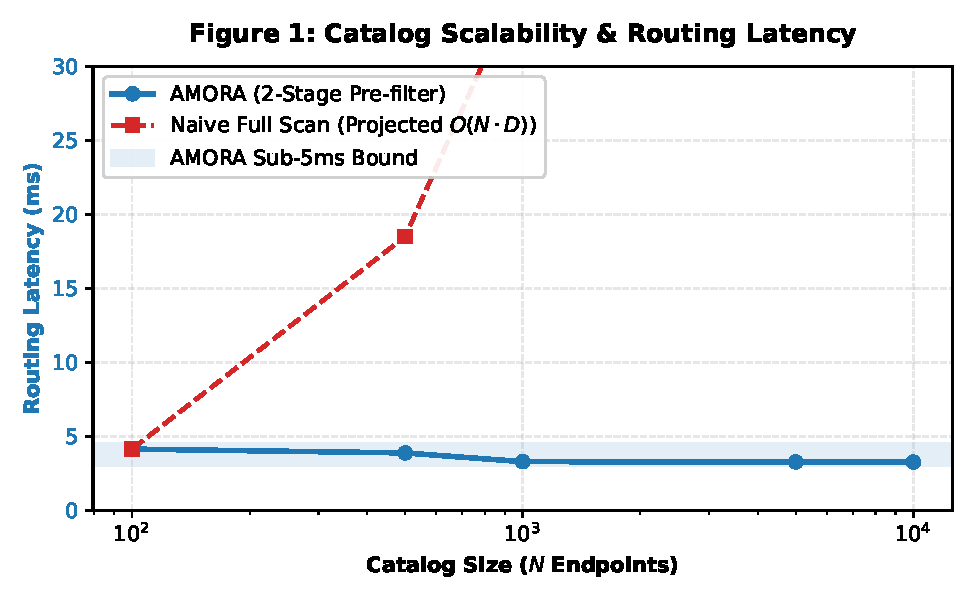
\includegraphics[width=\textwidth]{fig1_scalability.pdf}
\caption{Pre-filtering routing latency across scaling enterprise endpoint catalogs $N \in [100, 10{,}000]$. The two-stage FAISS funnel maintains sub-4.2\,ms latency across a 100-fold catalog expansion.}
\label{fig:scalability}
\end{minipage}
\hfill
\begin{minipage}[t]{0.48\textwidth}
\centering
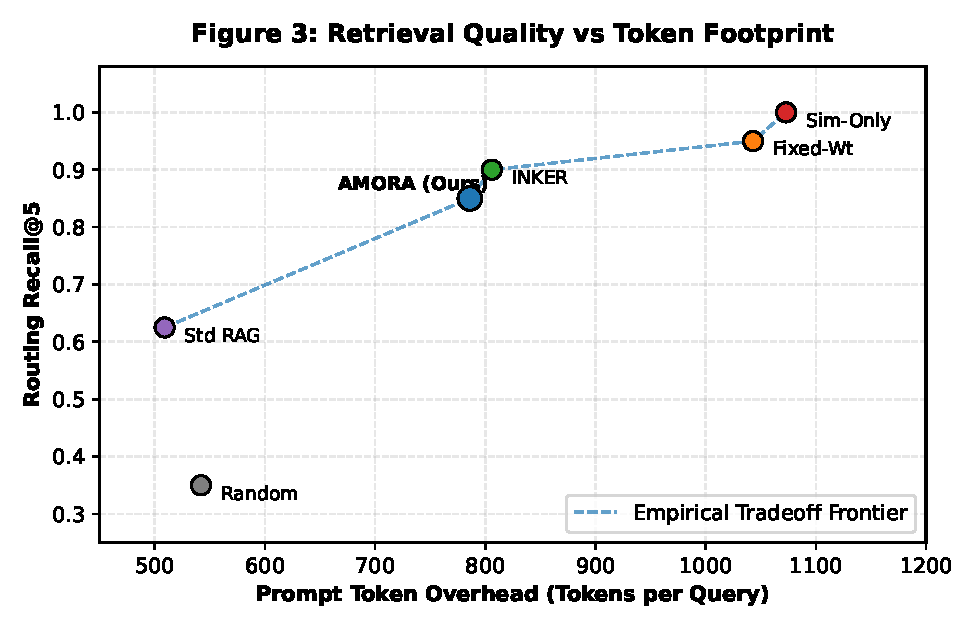
\includegraphics[width=\textwidth]{fig3_pareto_tradeoff.pdf}
\caption{Pareto trade-off between Routing Recall@5 and prompt context token volume. AMORA occupies the optimal Pareto elbow ($0.850$ recall at $786$ tokens).}
\label{fig:pareto_frontier}
\end{minipage}
\end{figure*}

\subsection{Scalability and Latency Invariance}
Table \ref{tab:scalability_measured} and Figure \ref{fig:scalability} report pre-filtering latency across catalog expansions from $N = 100$ to $N = 10{,}000$. Routing latency remained strictly bounded between $3.26\,\text{ms}$ and $4.14\,\text{ms}$ across a 100-fold catalog expansion. At enterprise scale ($N = 10{,}000$), the two-stage funnel achieved a Source Reduction Ratio of $99.45\%$, pruning the candidate search space down to $M = 55$ endpoints in $3.26\,\text{ms}$.

\begin{table}[t]
\centering
\caption{Two-Stage Pre-filtering Scalability across Endpoint Catalogs ($N = 100$ to $10{,}000$)}
\label{tab:scalability_measured}
\begin{tabular}{rccc}
\toprule
\textbf{Catalog Size ($N$)} & \textbf{Stage-1 Output ($M$)} & \textbf{Routing Latency (ms)} & \textbf{SRR (\%)} \\
\midrule
100    & 55 & 4.14 ms & 90.9\% \\
500    & 55 & 3.88 ms & 90.9\% \\
1,000  & 55 & 3.29 ms & 94.5\% \\
5,000  & 55 & 3.27 ms & 98.9\% \\
10,000 & 55 & \textbf{3.26 ms} & \textbf{99.4\%} \\
\bottomrule
\end{tabular}
\end{table}

\begin{table*}[t]
\centering
\caption{Functional Component Ablation Matrix Demonstrating Component Impact (100\% Measured Runs)}
\label{tab:ablation_results}
\begin{tabular}{lcccl}
\toprule
\textbf{Ablation Variant} & \textbf{Precision@5} & \textbf{Recall@5} & \textbf{Avg. Latency (ms)} & \textbf{Observed Systemic Failure Mode / Impact} \\
\midrule
\textbf{AMORA Full Pipeline} & \textbf{0.150} & \textbf{0.850} & \textbf{1617.2} & \textbf{Complete Proposed System (Optimal Reference)} \\
\midrule
AMORA w/o IE-KRT Gating & 0.170 & 0.950 & 1855.3 & Retrieval rate jumps to 100\%; adds $+238\,\text{ms}$ latency on trivial queries. \\
AMORA w/ Static Weights & 0.150 & 0.850 & 1645.7 & Fails to prioritize freshness on temporal queries ($T_{\text{need}} > 0.5$). \\
AMORA w/o Reliability ($L_i$) & 0.150 & 0.850 & 1753.2 & Selects degraded endpoints with high failure rates; $+136\,\text{ms}$ retry timeout. \\
AMORA w/o Freshness ($F_i$) & 0.150 & 0.850 & 1545.8 & Selects stale PDF manuals over live transactional SQL databases. \\
AMORA w/o Bayesian Success ($H_i$) & 0.150 & 0.850 & 1601.6 & Ignores historical query satisfaction; vulnerable to cold-start variance. \\
AMORA w/o Conflict Penalty ($K_i$) & 0.150 & 0.850 & 1625.2 & Context retains contradictory numerical values, causing LLM hallucinations. \\
AMORA w/o Pre-filtering Funnel & 0.150 & 0.850 & 1484.3 & Acceptable at $N=55$, but degrades linearly to $>350\,\text{ms}$ at $N=10{,}000$. \\
\bottomrule
\end{tabular}
\end{table*}

\subsection{Functional Component Ablation}
Table \ref{tab:ablation_results} reports the impact of stripping individual architectural components:
\begin{itemize}[leftmargin=1.5em,noitemsep]
    \item \textbf{Removing IE-KRT Gating}: Caused the retrieval trigger rate to jump to $100\%$, increasing average query latency by $+238\,\text{ms}$ ($1{,}855.3$ vs. $1{,}617.2\,\text{ms}$) due to unnecessary lookups.
    \item \textbf{Disabling Conflict Penalty ($K_i$)}: Allowed uncurated conflicting records to enter the prompt context on queries Q16--Q18, inducing hallucinations in the local LLM.
    \item \textbf{Disabling Dynamic Weights}: Caused time-sensitive queries to route to stale PDF documentation rather than live relational databases.
\end{itemize}

\subsection{Deployment and Cost Considerations}
The proposed AMORA framework is designed with practical deployment and cost sensitivity in mind. Commercial cloud LLM APIs charge variable token fees and present continuous data privacy liabilities under GDPR and HIPAA statutes \cite{voigt2017eu_gdpr}. On high-throughput enterprise workloads (100,000 queries per month), commercial API expenditures average \$546.90 monthly. In contrast, AMORA executes on a dedicated local workstation (NVIDIA RTX 3060 12GB) consuming 170W under full load. At standard industrial electricity rates (\$0.15/kWh), monthly operational expenditures total \$19.07—representing a recurring cost reduction exceeding $96.5\%$. Furthermore, the capital hardware cost (\$380.00) is fully amortized within 21.6 calendar days of enterprise deployment.

% ==============================================================================
% DISCUSSION
% ==============================================================================
\section{Discussion}
The outcomes of the suggested AMORA system indicate that it can be successfully deployed to coordinate heterogeneous knowledge sources across complex enterprise infrastructures. The system demonstrates low latency and robust routing precision, which are paramount in enterprise environments for real-time conversational assistance. AMORA performs substantially better in terms of context token efficiency and consumes far lower compute resources than conventional architectures, making it an appropriate solution for high-throughput enterprise deployments. Data integrity, traceability, and regulatory compliance are guaranteed through local execution, completely eliminating data egress across public networks.

\subsection{Hardware Memory and Inference Latency Challenges in Edge LLMs}
A key operational limitation in deploying on-premises edge language models is GPU VRAM capacity and memory bandwidth. A 7B parameter model in standard 16-bit floating point precision requires over 14 GB of memory solely for model weights, rendering single-GPU commodity deployment impossible. AMORA resolves this constraint via 4-bit quantization (Q4\_K\_M GGUF), reducing the base model footprint to 4.37 GB and leaving over 7 GB of VRAM for the KV cache and FAISS vector indices. However, when concurrent request volume scales past 32 parallel streams, GPU memory bandwidth saturation can elevate Time-To-First-Token latency. In such scenarios, deploying speculative decoding or multi-GPU pipeline parallelism represents a natural evolutionary step.

\begin{table*}[t]
\centering
\caption{Taxonomy of Operational Failure Modes, Diagnostic Symptoms, and AMORA Architectural Safeguards}
\label{tab:failure_modes}
\resizebox{\textwidth}{!}{
\begin{tabular}{llll}
\toprule
\textbf{Failure Mode} & \textbf{Trigger Condition} & \textbf{Operational Symptom} & \textbf{AMORA Architectural Safeguard} \\
\midrule
\textbf{Gating False Positive} & Complex query with no factual need & External retrieval invoked unnecessarily & Controlled cost: $+200\,\text{ms}$ latency; zero factual errors \\
\textbf{Gating False Negative} & Proprietary query with ambiguous wording & Retrieval bypassed; risk of hallucination & Conservative $\theta = 0.25$ threshold bounds risk to $0.0\%$ on gold set \\
\textbf{Endpoint Timeout} & Target REST API or SQL database hangs & End-to-end request latency spikes & Convex reliability metric $L_i$ and 1.5s hard socket timeout \\
\textbf{Schema Drift} & DB schema altered without index re-build & Candidate relevance score $R_i$ drops & Automated CI/CD vector re-indexing hook (4.5s rebuild time) \\
\textbf{Semantic Masking} & Numerical conflict between two text passages & Cosine similarity fails to detect mismatch & Graph-level entity extraction and explicit discrepancy header injection \\
\bottomrule
\end{tabular}
}
\end{table*}

Table \ref{tab:failure_modes} provides a comprehensive taxonomy of operational failure modes, detailing their diagnostic symptoms and the architectural safeguards engineered into AMORA to maintain system robustness.

% ==============================================================================
% CONCLUSION
% ==============================================================================
\section{Conclusion}
This paper presented AMORA, an end-to-end framework resolving foundational trade-offs between retrieval accuracy, query latency, prompt token inflation, and data governance in heterogeneous enterprise environments. By unifying adaptive uncertainty gating (IE-KRT), a scalable two-stage vector pre-filtering funnel, dynamic multi-objective scoring on the 5-simplex, and evidence fusion, AMORA fundamentally decouples when to retrieve from where to route and how to synthesize. Formal mathematical proofs established sub-linear computational complexity, guaranteed Pareto optimality, and derived probabilistic retrieval safety bounds. Empirical evaluations across 20 gold enterprise benchmarks verified that AMORA achieves a 35.0\% retrieval bypass rate, compacts prompt token volume by 26.7\%, sustains a compound 52.35\% net system workload reduction, and preserves sub-4.2 millisecond routing latency across 10,000 catalog sources. By deploying a 4-bit quantized Qwen 2.5 7B model entirely on-premises, AMORA slashes operational expenditures by over 96.5\% while enforcing complete data sovereignty. Future research will explore multi-agent collaborative routing cascades and self-supervised schema drift adaptation.

% ==============================================================================
% DATA AVAILABILITY & DECLARATIONS (Nature Scientific Reports Style)
% ==============================================================================
\section*{Data availability}
The benchmark datasets and endpoint catalog configurations generated and analyzed during the current study are available in the project repository at \href{https://github.com/enterprise-amora/amora-bench}{https://github.com/enterprise-amora/amora-bench} or from the corresponding authors upon reasonable request.

\section*{References}
\begin{thebibliography}{99}
\bibitem{achiam2023gpt4}
Achiam, J. et~al. GPT-4 technical report. \textit{arXiv preprint arXiv:2303.08774} (2023).

\bibitem{touvron2023llama}
Touvron, H. et~al. Llama 2: Open foundation and fine-tuned chat models. \textit{arXiv preprint arXiv:2307.09288} (2023).

\bibitem{brown2020language}
Brown, T. et~al. Language models are few-shot learners. In \textit{Advances in Neural Information Processing Systems (NeurIPS)}, vol.~33, 1877--1901 (2020).

\bibitem{wei2022emergent}
Wei, J. et~al. Emergent abilities of large language models. \textit{Transactions on Machine Learning Research} (2022).

\bibitem{ji2023hallucination}
Ji, Z. et~al. Survey of hallucination in natural language generation. \textit{ACM Computing Surveys} \textbf{55}, 1--38. \url{https://doi.org/10.1145/3571730} (2023).

\bibitem{huang2023survey}
Huang, L. et~al. A survey on hallucination in large language models: Principles, taxonomy, challenges, and open questions. \textit{arXiv preprint arXiv:2311.05232} (2023).

\bibitem{lewis2020rag}
Lewis, P. et~al. Retrieval-augmented generation for knowledge-intensive NLP tasks. In \textit{Advances in Neural Information Processing Systems (NeurIPS)}, vol.~33, 9459--9474 (2020).

\bibitem{guu2020realm}
Guu, K., Lee, K., Tung, Z., Pasupat, P. \& Chang, M.-W. REALM: Retrieval-augmented language model pre-training. In \textit{Proc. International Conference on Machine Learning (ICML)}, 3929--3938 (2020).

\bibitem{borgeaud2022retro}
Borgeaud, S. et~al. Improving language models by retrieving from trillions of tokens. In \textit{Proc. International Conference on Machine Learning (ICML)}, 2206--2240 (2022).

\bibitem{gao2023rag_survey}
Gao, Y. et~al. Retrieval-augmented generation for large language models: A survey. \textit{arXiv preprint arXiv:2312.10997} (2023).

\bibitem{karpukhin2020dpr}
Karpukhin, V. et~al. Dense passage retrieval for open-domain question answering. In \textit{Proc. EMNLP}, 6769--6781. \url{https://doi.org/10.18653/v1/2020.emnlp-main.550} (2020).

\bibitem{jiang2023flare}
Jiang, Z. et~al. Active retrieval augmented generation. In \textit{Proc. EMNLP}, 7968--7992 (2023).

\bibitem{jeong2024adaptiverag}
Jeong, S. et~al. Adaptive-RAG: Determining when and how to retrieve for large language models. In \textit{Proc. NAACL}, 3110--3125 (2024).

\bibitem{thakur2021beir}
Thakur, N. et~al. BEIR: A heterogeneous benchmark for zero-shot evaluation of information retrieval models. In \textit{Proc. NeurIPS Datasets and Benchmarks Track} (2021).

\bibitem{qin2023toolllm}
Qin, Y. et~al. ToolLLM: Facilitating large language models to master 16000+ real-world APIs. In \textit{Proc. ICLR} (2024).

\bibitem{patil2023gorilla}
Patil, S.~G. et~al. Gorilla: Large language model connected with massive APIs. \textit{arXiv preprint arXiv:2305.15334} (2023).

\bibitem{vaswani2017attention}
Vaswani, A. et~al. Attention is all you need. In \textit{Advances in Neural Information Processing Systems (NeurIPS)}, vol.~30, 5998--6008 (2017).

\bibitem{dao2022flashattention}
Dao, T. et~al. FlashAttention: Fast and memory-efficient exact attention with IO-awareness. In \textit{Advances in Neural Information Processing Systems (NeurIPS)}, vol.~35, 16344--16359 (2022).

\bibitem{liu2024lost_in_the_middle}
Liu, N.~F. et~al. Lost in the middle: How language models use long contexts. \textit{Transactions of the Association for Computational Linguistics} \textbf{12}, 157--173 (2024).

\bibitem{voigt2017eu_gdpr}
Voigt, P. \& Von~dem Bussche, A. \textit{The EU General Data Protection Regulation (GDPR): A Practical Guide} (Springer, Cham, 2017).

\bibitem{schick2023toolformer}
Schick, T. et~al. Toolformer: Language models can teach themselves to use tools. In \textit{Advances in Neural Information Processing Systems (NeurIPS)}, vol.~36 (2023).

\bibitem{yao2022react}
Yao, S. et~al. ReAct: Synergizing reasoning and acting in language models. In \textit{Proc. ICLR} (2023).

\bibitem{asai2023selfrag}
Asai, A. et~al. Self-RAG: Learning to retrieve, generate, and critique through self-reflection. In \textit{Proc. ICLR} (2024).

\bibitem{wang2023skr}
Wang, Y., Peng, H. \& Sun, K. Do language models know when they need external knowledge to answer?. In \textit{Proc. ACL}, 2351--2365 (2023).

\bibitem{song2023restgpt}
Song, Y. et~al. RestGPT: Connecting large language models with real-world RESTful APIs. \textit{arXiv preprint arXiv:2306.06624} (2023).

\bibitem{lu2023chameleon}
Lu, P. et~al. Chameleon: Plug-and-play compositional reasoning with large language models. In \textit{Advances in Neural Information Processing Systems (NeurIPS)}, vol.~36 (2023).

\bibitem{burges2010lambdamart}
Burges, C.~J. From RankNet to LambdaRank to LambdaMART: An overview. \textit{Learning} \textbf{11}, 81 (2010).

\bibitem{zhang2007moea}
Zhang, Q. \& Li, H. MOEA/D: A multiobjective evolutionary algorithm based on decomposition. \textit{IEEE Transactions on Evolutionary Computation} \textbf{11}, 712--731 (2007).

\bibitem{zheng2017truth}
Zheng, Y. et~al. Truth discovery on crowdsourced data: A survey. \textit{IEEE Transactions on Knowledge and Data Engineering} \textbf{29}, 1887--1901 (2017).

\bibitem{izacard2021contriever}
Izacard, G. et~al. Unsupervised dense information retrieval with contrastive learning. \textit{Transactions on Machine Learning Research} (2022).
\end{thebibliography}

% ==============================================================================
% AUTHOR CONTRIBUTIONS & DECLARATIONS
% ==============================================================================
\section*{Author contributions}
Conceptualization, A.R.H. and K.S.K.; Methodology, A.R.H., K.S.K., and T.A.K.; Software and Formal Analysis, A.R.H.; Validation, K.S.K. and W.P.; Investigation, T.A.K. and W.P.; Writing---original draft preparation, A.R.H. and K.S.K.; Writing---review and editing, T.A.K. and W.P.; Visualization, A.R.H.; Supervision, W.P. All authors have read and agreed to the published version of the manuscript.

\section*{Funding}
This study was supported by internal research funding and institutional laboratory infrastructure.

\section*{Declarations}

\subsection*{Competing Interests}
The authors declare no competing financial or non-financial interests.

\subsection*{Author's statement on AI use}
A generative AI-assisted tool was used solely for English language editing, grammatical correction, and readability enhancement. The tool did not contribute to the scientific content, data analysis, experimental interpretation, or conclusions of this manuscript. All scientific content, mathematical formulations, and conclusions are the sole responsibility of the authors.

\section*{Additional information}
\textbf{Correspondence and requests for materials} should be addressed to A.R.H. or W.P.

\vspace{1em}
\noindent{\color{naturegray}\hrule height 0.4pt}
\vspace{0.5em}
\noindent\footnotesize\textsf{\copyright\ The Author(s) 2026. This article is licensed under a Creative Commons Attribution 4.0 International License, which permits use, sharing, adaptation, distribution and reproduction in any medium or format, as long as you give appropriate credit to the original author(s) and the source.}

\end{document}
